\documentclass{article}

\usepackage{amsmath}
\usepackage{mathtools}
\usepackage{amsfonts} 
\usepackage{geometry}
\usepackage{soul}
\usepackage{indentfirst}
\usepackage{multicol}
\usepackage{tikz}
\usetikzlibrary{calc, automata, chains, arrows.meta, math}



\title{A game theoretic model of the behavioural gaming that takes place at the EMS - ED interface}
\author{}
\date{}

\begin{document}
\maketitle


\begin{figure}[h]
    \centering
    \begin{tikzpicture}[-, node distance = 3cm, auto]
        \node[anchor=north](H1){\(H_1\)};
        \node[anchor=north](H1_d1) at (3, 2){.};
        \node[anchor=north](H1_d2) at (3, -2){.};

        \path(H1) edge node {}(H1_d1);
        \path(H1) edge node {}(H1_d2);
        \path(H1_d1) edge [bend left] node {}(H1_d2);
        \path(H1_d1) [dashed] edge node {}(H1_d2);

        \node[anchor=north](H2) at (3.9, 0){\(H_2\)};
        \node[anchor=north](H2_d1) at (6.9, 2){.};
        \node[anchor=north](H2_d2) at (6.9, -2){.};

        \path(H2) edge node {}(H2_d1);
        \path(H2) edge node {}(H2_d2);
        \path(H2_d1) edge [bend left] node {}(H2_d2);

        \node[anchor=north](A) at (7.8, 0){\(A\)};
        \node[anchor=north](A_d1) at (10.8, 2){.};
        \node[anchor=north](A_d2) at (10.8, -2){.};
        
        \path(A) edge node {}(A_d1);
        \path(A) edge node {}(A_d2);
        \path(A_d1) edge [bend left] node {}(A_d2);

    \end{tikzpicture}
    \caption{Ambulance Decision Problem} 
    \label{Ambulance_Problem}
\end{figure}

{\Large\textbf{States:}}

\begin{enumerate}
    \item \(A\) = Ambulance
    \item \(H_i\) = Hospital i
\end{enumerate}

{\Large\textbf{Notation:}}
\begin{itemize}
    \item \(\Lambda\) = total number of patients that need to be hospitalised
    \item \(p_i\) = proportion of patients going to Hospital i (\(p_i\Lambda\) = number of patients going to hospital i)
    \item \(d_i\) = distance from Hospital i
    \item \(\hat{c_i}\) = capacity of hospital i
    \item \(W(c, \lambda\, \mu)\) = waiting time in the system function
    \item \(\mu_i\) = service rate of hospital i
    \item \(\lambda_i^o\) = arrival rate of other patients to the hospital (not by ambulance)
    \item \(C_i(p_i) = d_i + W(c = \hat{c_i},\hspace{0.1cm} \lambda = p_i\Lambda + \lambda_i^o, \hspace{0.1cm} \mu = \mu_i)\)
\end{itemize}

\newpage

\section{Game Theory component:} 
\textbf{\underline{Players:}} 
\begin{itemize}
    \item Ambulance
    \item Hospital A
    \item Hospital B
\end{itemize}

\noindent 
\textbf{\underline{Strategies of players:}}
\begin{itemize}
    \item Hospital i:    
    \begin{enumerate} 
        \item Close doors at $\hat{c_i} = 1$ 
        \item Close doors at $\hat{c_i} = 2$
        \item \dots
        \item Close doors at $\hat{c_i} = C_i$
    \end{enumerate}
    \item Ambulance:
    \begin{enumerate}
        \item Choose $p_1 \in [0,1]$ 
    \end{enumerate}
\end{itemize}

\noindent 
\textbf{\underline{Cost Functions:}} Waiting times + the distance to each hospital. 





% \section{Queuing Theory component}

% The waiting times are functions dependent to the service rate ($\mu$), the arrival rate ($\lambda$) and the hospital's capacity. Thus, for every instance of the routing game (i.e. for every different value of $p_1$ and $p_2$) a new waiting time value will be calculated. The mean waiting time in the queue for an $M|M|c$ system is defined as:



\section{Formulas}
$$\hat{c_i} \in \{1,2, \dots, C_i\} $$
$$ \rho_i = \frac{p_i \Lambda + \lambda_i^o}{\hat{c_i}\mu_i} $$
$$ (W_q)_i = \frac{1}{\hat{c_i} \mu_i} \frac{(\hat{c_i} \rho_i)^{\hat{c_i}}}{\hat{c_i}!(1-\rho_i)^2}(P_0)_i $$
$$ (P_0)_i = \frac{1}{\sum_{n = 0}^{\hat{c_i} - 1} \left[ \frac{(\hat{c_i} \rho_i)^n}{n!} \right] + \frac{(\hat{c_i}\rho_i)^{\hat{c_i}}}{\hat{c_i}!(1-\rho_i)}} $$

\newpage
\section{Quick Methodology}

\begin{itemize}
    \item Fix the parameters $\Lambda$, $\lambda_i^o$, $\mu_i$ and $C_i$. 
    \item $\forall \hspace{0.2cm} \hat{c_i} \in \{1,2, \dots, C_A\}$ and $\forall \hspace{0.2cm} \hat{c_j} \in \{1,2, \dots, C_B\}$ 
    \item Calculate $p_A$ and $p_B = 1-p_A$ s.t. $(W_q)_A = (W_q)_B$. 
    \item Calculate the probability $P((W_q)_i \leq 4$ hours
    \item Fill matrix A with $ U_{\hat{c_i}, \hat{c_j}}^A = 1 - |0.95 - P((W_q)_A \leq 4)|$ and
    \item fill matrix B with $ U_{\hat{c_i}, \hat{c_j}}^B = 1 - |0.95 - P((W_q)_B \leq 4)| $
\end{itemize}



\begin{table}[h]
    \centering
    A = 
    \begin{tabular}{|l|l|l|l|}
    \hline
    $U_{1,1}^A$ & $U_{1,2}^A$ & \dots & $U_{1,C_B}^A$ \\ \hline
    $U_{2,1}^A$ & $U_{2,2}^A$ & \dots & $U_{2,C_B}^A$ \\ \hline
    \vdots & \vdots & $\ddots$ & \vdots \\ \hline
    $U_{C_A,1}^A$ & $U_{C_A,2}^A$ & \dots & $U_{C_A,C_B}^A$ \\ \hline
    \end{tabular}
\end{table}  

\begin{table}[h]
    \centering
    B = 
    \begin{tabular}{|l|l|l|l|}
    \hline
    $U_{1,1}^B$ & $U_{1,2}^B$ & \dots & $U_{1,C_B}^B$ \\ \hline
    $U_{2,1}^B$ & $U_{2,2}^B$ & \dots & $U_{2,C_B}^B$ \\ \hline
    \vdots & \vdots & $\ddots$ & \vdots \\ \hline
    $U_{C_A,1}^B$ & $U_{C_A,2}^B$ & \dots & $U_{C_A,C_B}^B$ \\ \hline
    \end{tabular}
\end{table}  

\begin{itemize}
    \item Ambulance decides the proportion of people to distribute to each hospital based on optimal patient distribution.
\end{itemize}


\section{Distribution of waiting time}
\begin{equation}
    P(W_q > T) = \frac{(\frac{\lambda}{\mu})^c P_0}{c!(1-\frac{\lambda}{c \mu})} (e^{-(c \mu - \lambda)T})
\end{equation}



\newpage
\section{Proper Methodology}
The problem is formulated as a normal form game where the players are the two hospitals. Each hospital is given $C_A$ and $C_B$ number of strategies where $C_A$ and $C_B$ are the total capacities of the hospitals. In other words, depending on the capacity of each hospital, they may choose to stop receiving patients from arriving ambulances whenever they reach a certain capacity threshold. The goal of this problem is to satisfy the ED regulations which state that 95\% of the patients should see a specialist within 4 hours of their arrival to the hospital. The mean of the random variable $W_q$ is the average waiting time in the queue for hospital i.


\begin{equation}
     W_q(\lambda_i, \mu_i, \hat{c_i}) = \frac{1}{\hat{c_i} \mu_i} \frac{(\hat{c_i} \rho_i) ^ {\hat{c_i}}}{\hat{c_i}! (1 - \rho_i) ^ 2}P_0, \quad i \in \{A,B\}
\end{equation}

Thus, the utilities of the two players should be the proportion of people that fall within the 4 hours target. This is also equivalent to the probability of the waiting time of an individual to be less than or equal to 4 hours. 

\begin{equation}
    P(W_q(\lambda_i, \mu_i, \hat{c_i}) \leq 4), \quad i \in \{A,B\}
\end{equation}

Therefore, a sensible goal for each player should be to minimise that probability, but the actual target of the hospitals is to satisfy 95\% of those patients within the 4-hour time limit. Therefore, the goal should be to get that probability as close to 0.95 as possible. Thus each player should aim to minimise:

\begin{equation}
    |0.95 - P(W_q(\lambda_i, \mu_i, \hat{c_i}) \leq 4)|, \quad i \in \{A,B\}
\end{equation}

The classic formulation of a normal form game looks into the maximisation of each player's payoff. Consequently the utilities can be altered such that the goal of each player is to maximise:

\begin{align}\label{Utilities}
    U_{\hat{c_A}, \hat{c_B}} ^ {A} = 1 - |0.95 - P(W_q(\lambda_A, \mu_A, \hat{c_A}) \leq 4)| \\
    U_{\hat{c_A}, \hat{c_B}} ^ {B} = 1 - |0.95 - P(W_q(\lambda_B, \mu_B, \hat{c_B}) \leq 4)|
\end{align}

Finally, the problem can be expressed as a normal form game with two players where each player/hospital has $C_A$ and $C_B$ strategies respectively. The two $C_A \times C_B$ payoff matrices for the utilities of the two hospitals can be defined as:

\begin{table}[h]
    \centering
    \begin{minipage}{.5\linewidth}
        A = 
        \begin{tabular}{|l|l|l|l|}
            \hline
            $U_{1,1}^A$ & $U_{1,2}^A$ & \dots & $U_{1,C_2}^A$ \\ \hline
            $U_{2,1}^A$ & $U_{2,2}^A$ & \dots & $U_{2,C_2}^A$ \\ \hline
            \vdots & \vdots & $\ddots$ & \vdots \\ \hline
            $U_{C_1,1}^A$ & $U_{C_1,2}^A$ & \dots & $U_{C_1,C_2}^A$ \\ \hline
        \end{tabular}
    \end{minipage}%
    \begin{minipage}{.5\linewidth}
        B = 
        \begin{tabular}{|l|l|l|l|}
            \hline
            $U_{1,1}^B$ & $U_{1,2}^B$ & \dots & $U_{1,C_2}^B$ \\ \hline
            $U_{2,1}^B$ & $U_{2,2}^B$ & \dots & $U_{2,C_2}^B$ \\ \hline
            \vdots & \vdots & $\ddots$ & \vdots \\ \hline
            $U_{C_1,1}^B$ & $U_{C_1,2}^B$ & \dots & $U_{C_1,C_2}^B$ \\ \hline
        \end{tabular}
    \end{minipage}
\end{table}  
Once the certain strategies of the game have been selected the ambulance service can decide what would be the optimal way to distribute patients. However, the way the ambulance service distributes patients can affect the utilities of the game. So how would one solve this kind of problem?
 
\subsection{Solution}
As mentioned before the problem requires the construction of two queuing models that will be needed for the formulation of the normal form game. Based on those utilities the ambulance service will then decide the percentage of patients that will distribute to each hospital. 

First and foremost, the model consists of several parameters that are unknown and are assumed to be fixed. The model will be run multiple times for various values of these parameters.


\begin{table}[h]
    \centering
    \begin{tabular}{|l|l|}
        \hline
        $\Lambda$ & Number of patients that need to be distributed \\ \hline
        $\lambda_i^o$ & Arrival rate of other patients that enter hospital i \\ \hline
        $\mu_i$ & Service rate of hospital i \\ \hline
        $C_i$ & Total capacity of hospital i \\ \hline
    \end{tabular}
    \caption{Fixed Parameters}
\end{table}

Having established the fixed parameters of the model, the hospitals' utilities need to be calculated. In order to do so a backwards induction approach will be used. The EMS aims to distribute the patients such that the mean waiting time of patients is minimal. This can be further interpreted as when the mean waiting time of hospital A equals the mean waiting time of hospital B. Thus, the minimal mean waiting time can be found for the values of $p_A$ and $p_B$ that solve the following equation:

\begin{equation}\label{Equal_Wait}
    W_q(\lambda_A, \mu_A, \hat{c_A}) = W_q(\lambda_B, \mu_B, \hat{c_B})
\end{equation}

Equation (\ref{Equal_Wait}) needs to be solved for all values of $c_i \in \{1,2, \dots C_A\}$ and $c_j \in \{1,2, \dots C_B\}$. Then, for every $c_i$ and $c_j$ the utility equation (\ref{Utilities}) has to be calculated for both hospitals. In order to solve it though, one must first estimate the probability $P[(W_q)_{\{A, B\}}] \leq 4]$. That is the probability that the waiting time in the queue for one of the hospitals is less than 4 hours. For a multi-server system, the distribution of the waiting time can be given by equation \ref{Dist_Wait}. The above expression returns the probability that the waiting time in the queue is less than some time T.

\begin{equation}\label{Dist_Wait}
    P(W_q > T) = \frac{(\frac{\lambda}{\mu})^c P_0}{c!(1-\frac{\lambda}{c \mu})} (e^{-(c \mu - \lambda)T})
\end{equation}

Consequently when incorporating equation (\ref{Dist_Wait}) into (\ref{Utilities}) a newer utility equation can be acquired:
 
\begin{equation}\label{Utilities2}
    U_{\hat{c_i}, \hat{c_j}} ^ {\{A, B\}} = 1 - \left| \left[ \frac{(\frac{\lambda}{\mu})^c P_0}{c!(1-\frac{\lambda}{c \mu})} \left( e^{-(c \mu - \lambda)T} \right) \right] - 0.05 \right|
\end{equation}

\begin{table}[h]
    \centering
    \begin{minipage}{.5\linewidth}
        A = 
        \begin{tabular}{|l|l|l|l|}
            \hline
            $U_{1,1}^A$ & $U_{1,2}^A$ & \dots & $U_{1,C_2}^A$ \\ \hline
            $U_{2,1}^A$ & $U_{2,2}^A$ & \dots & $U_{2,C_2}^A$ \\ \hline
            \vdots & \vdots & $\ddots$ & \vdots \\ \hline
            $U_{C_1,1}^A$ & $U_{C_1,2}^A$ & \dots & $U_{C_1,C_2}^A$ \\ \hline
        \end{tabular}
    \end{minipage}%
    \begin{minipage}{.5\linewidth}
        B = 
        \begin{tabular}{|l|l|l|l|}
            \hline
            $U_{1,1}^B$ & $U_{1,2}^B$ & \dots & $U_{1,C_2}^B$ \\ \hline
            $U_{2,1}^B$ & $U_{2,2}^B$ & \dots & $U_{2,C_2}^B$ \\ \hline
            \vdots & \vdots & $\ddots$ & \vdots \\ \hline
            $U_{C_1,1}^B$ & $U_{C_1,2}^B$ & \dots & $U_{C_1,C_2}^B$ \\ \hline
        \end{tabular}
    \end{minipage}
\end{table}  





% \newgeometry{left=0.6cm, right=0.4cm}
\section{Markov Chain Representation of Hospital}
The following Markov chain represents the transition between states of a hospital while capturing the EMS interaction with it. The hospital accepts both ambulance and other patients normally until a certain threshold $T$ is reached. When it is reached all ambulances that arrive will be marked as \textit{"parked outside"} until the number of people in the system is reduced below $T$. Alternatively, if the patients in the system keep rising, they may reach the total capacity $C$ of the hospital and the other patients will be waiting for until a service becomes free. The states of the Markov chain are denoted by $(u,v)$ where:
\begin{itemize}
    \item $u$ = number of ambulances parked outside of the hospital
    \item $v$ = number of patients in the hospital
\end{itemize}


\begin{figure}[h]
    \centering
    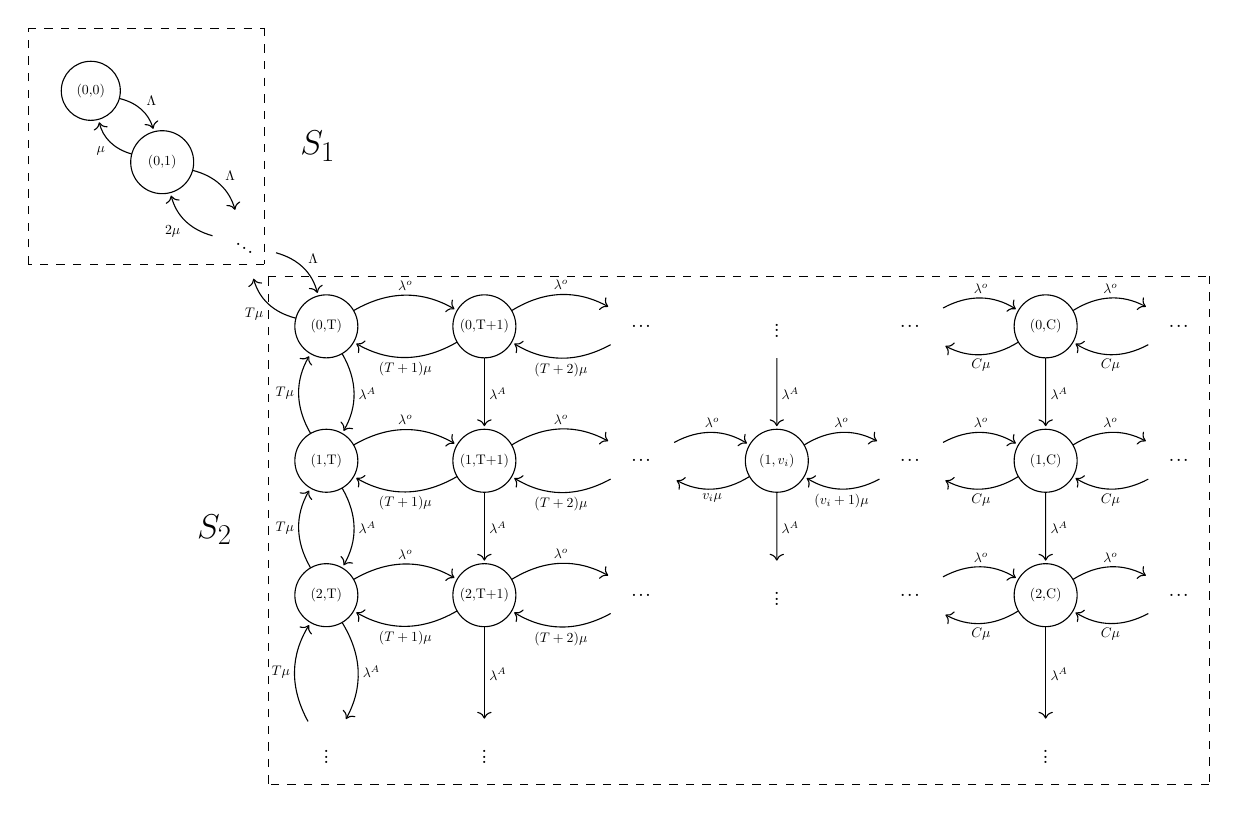
\begin{tikzpicture}[-, node distance = 0.9cm, auto, every node/.style={scale=0.5}]

        % Variables
        \tikzmath{
            let \initdist = 0.5cm;
            let \altdist = 1.2cm;
            let \minsz = 1.6cm;
            let \leftOne = -0.8;
            let \rightOne = 2.2;
            let \upOne = 0.8;
            let \downOne = -2.2;
            let \leftTwo = 2.25;
            let \rightTwo = 14.2;
            let \upTwo = -2.35;
            let \downTwo = -8.8;
        }

        % Rectangle for S1
        \draw[ultra thin, dashed] (\leftOne, \downOne) -- (\leftOne, \upOne);
        \draw[ultra thin, dashed] (\leftOne, \upOne) -- (\rightOne, \upOne);
        \draw[ultra thin, dashed] (\rightOne, \upOne) -- node {\Huge{$\quad S_1$}}(\rightOne, \downOne);
        \draw[ultra thin, dashed] (\rightOne, \downOne) -- (\leftOne, \downOne);

        % Rectangle for S2
        \draw[ultra thin, dashed] (\leftTwo, \downTwo) -- node {\Huge{$S_2 \quad$}}(\leftTwo, \upTwo);
        \draw[ultra thin, dashed] (\leftTwo, \upTwo) -- (\rightTwo, \upTwo);
        \draw[ultra thin, dashed] (\rightTwo, \upTwo) -- (\rightTwo, \downTwo);
        \draw[ultra thin, dashed] (\rightTwo, \downTwo) -- (\leftTwo, \downTwo);

        % First Line
        \node[state, minimum size=1.5cm] (zero) {(0,0)};
        \node[state, node distance = \initdist, minimum size=\minsz, below right=of zero] (one) {(0,1)};
        \node[draw=none, node distance = \initdist, minimum size=\minsz, below right=of one] (two) {\textbf{$\ddots$}};
        \node[state, node distance = \initdist, minimum size=\minsz, below right=of two] (three) {(0,T)};
        \node[state, node distance = \altdist, minimum size=\minsz, right=of three] (four) {(0,T+1)};
        \node[draw=none, node distance = \altdist, minimum size=\minsz, right=of four] (five) {\textbf{\dots}};
        \node[draw=none, minimum size=\minsz, right=of five] (six) {\textbf{\vdots}};
        \node[draw=none, minimum size=\minsz, right=of six] (seven) {\textbf{\dots}};
        \node[state, minimum size=\minsz, right=of seven] (eight) {(0,C)};
        \node[draw=none, minimum size=\minsz, right=of eight] (nine) {\textbf{\dots}};


        % Second Line
        \node[state, minimum size=\minsz, below=of three] (three_one) {(1,T)};
        \node[state, minimum size=\minsz, below=of four] (four_one) {(1,T+1)};
        \node[draw=none, minimum size=\minsz, below=of five] (five_one) {\textbf{\dots}};
        \node[state, minimum size=\minsz, right=of five_one] (six_one) {$(1, v_i)$};
        \node[draw=none, minimum size=\minsz, right=of six_one] (seven_one) {\textbf{\dots}};
        \node[state, minimum size=\minsz, right=of seven_one] (eight_one) {(1,C)};
        \node[draw=none, minimum size=\minsz, right=of eight_one] (nine_one) {\textbf{\dots}};
        

        % Third Line
        \node[state, minimum size=\minsz, below=of three_one] (three_two) {(2,T)};
        \node[state, minimum size=\minsz, below=of four_one] (four_two) {(2,T+1)};
        \node[draw=none, minimum size=\minsz, below=of five_one] (five_two) {\textbf{\dots}};
        \node[draw=none, minimum size=\minsz, right=of five_two] (six_two) {\textbf{\vdots}};
        \node[draw=none, minimum size=\minsz, right=of six_two] (seven_two) {\textbf{\dots}};
        \node[state, minimum size=\minsz, right=of seven_two] (eight_two) {(2,C)};
        \node[draw=none, minimum size=\minsz, right=of eight_two] (nine_two) {\textbf{\dots}};

        % Fourth line
        \node[draw=none, node distance = \altdist, minimum size=\minsz, below=of three_two] (three_three) {\textbf{\vdots}};
        \node[draw=none, node distance = \altdist, minimum size=\minsz, below=of four_two] (four_three) {\textbf{\vdots}};
        \node[draw=none, node distance = \altdist, minimum size=\minsz, below=of five_two] (five_three) {};
        \node[draw=none, node distance = \altdist, minimum size=\minsz, below=of six_two] (six_three) {};
        \node[draw=none, node distance = \altdist, minimum size=\minsz, below=of eight_two] (eight_three) {\textbf{\vdots}};


        \draw[every loop]
            % First Horizontal Edges
            (zero) edge[bend left] node {$\Lambda$} (one)
            (one) edge[bend left] node {$\mu$} (zero)
            (one) edge[bend left] node {$\Lambda$} (two)
            (two) edge[bend left] node {$2 \mu$} (one)
            (two) edge[bend left] node {$\Lambda$} (three)
            (three) edge[bend left] node {$T \mu$} (two)
            (three) edge[bend left] node {$\lambda^o$} (four)
            (four) edge[bend left] node {$(T+1) \mu$} (three)
            (four) edge[bend left] node {$\lambda^o$} (five)
            (five) edge[bend left] node {$(T+2) \mu$} (four)
            % (five) edge[bend left] node {$\lambda^o$} (six)
            % (six) edge[bend left] node [above] {$C\mu$} (five)
            % (six) edge[bend left] node {$\lambda^o$} (seven)
            % (seven) edge[bend left] node [above] {$C\mu$} (six)
            (seven) edge[bend left] node {$\lambda^o$} (eight)
            (eight) edge[bend left] node {$C\mu$} (seven)
            (eight) edge[bend left] node {$\lambda^o$} (nine)
            (nine) edge[bend left] node {$C\mu$} (eight)

            % Second Horizontal Edges
            (three_one) edge[bend left] node {$\lambda^o$} (four_one)
            (four_one) edge[bend left] node {$(T+1) \mu$} (three_one)
            (four_one) edge[bend left] node {$\lambda^o$} (five_one)
            (five_one) edge[bend left] node {$(T+2) \mu$} (four_one)
            (five_one) edge[bend left] node {$\lambda^o$} (six_one)
            (six_one) edge[bend left] node {$v_i\mu$} (five_one)
            (six_one) edge[bend left] node {$\lambda^o$} (seven_one)
            (seven_one) edge[bend left] node {$(v_i+1)\mu$} (six_one)
            (seven_one) edge[bend left] node {$\lambda^o$} (eight_one)
            (eight_one) edge[bend left] node {$C\mu$} (seven_one)
            (eight_one) edge[bend left] node {$\lambda^o$} (nine_one)
            (nine_one) edge[bend left] node {$C\mu$} (eight_one)

            % Third Horizontal Edges
            (three_two) edge[bend left] node {$\lambda^o$} (four_two)
            (four_two) edge[bend left] node [below] {$(T+1) \mu$} (three_two)
            (four_two) edge[bend left] node {$\lambda^o$} (five_two)
            (five_two) edge[bend left] node {$(T+2) \mu$} (four_two)
            % (five_two) edge[bend left] node {$\lambda^o$} (six_two)
            % (six_two) edge[bend left] node [above] {$C\mu$} (five_two)
            % (six_two) edge[bend left] node {$\lambda^o$} (seven_two)
            % (seven_two) edge[bend left] node [above] {$C\mu$} (six_two)
            (seven_two) edge[bend left] node {$\lambda^o$} (eight_two)
            (eight_two) edge[bend left] node {$C\mu$} (seven_two)
            (eight_two) edge[bend left] node {$\lambda^o$} (nine_two)
            (nine_two) edge[bend left] node {$C\mu$} (eight_two)

            % First Vertical Edges
            (three) edge[bend left] node {$\lambda^A$} (three_one)
            (three_one) edge[bend left] node {$T \mu$} (three)
            (three_one) edge[bend left] node {$\lambda^A$} (three_two)
            (three_two) edge[bend left] node {$T\mu$} (three_one)
            (three_two) edge[bend left] node {$\lambda^A$} (three_three)
            (three_three) edge[bend left] node {$T\mu$} (three_two)

            % Second Vertical Edges
            (four) edge node {$\lambda^A$} (four_one)
            (four_one) edge node {$\lambda^A$} (four_two)
            (four_two) edge node {$\lambda^A$} (four_three)

            % Third Vertical Edges
            (six) edge node {$\lambda^A$} (six_one)
            (six_one) edge node {$\lambda^A$} (six_two)
            % (six_two) edge node {$\lambda^A$} (six_three)

            % Fourth Vertical Edges
            (eight) edge node {$\lambda^A$} (eight_one)
            (eight_one) edge node {$\lambda^A$} (eight_two)
            (eight_two) edge node {$\lambda^A$} (eight_three)
            ;       
    \end{tikzpicture}
    \caption{Markov chains} 
    \label{markov_model}
\end{figure}

\subsection{Markov-chain state mapping function}
The transition matrix of the Markov-chain representation described above can be denoted by a state mapping function. The state space of this function is defined as:



\begin{align}
    S(T) =& S_1(T) \cup S_2(T) \text{ where:} \nonumber \\
    S_1(T) =& \left\{(0, v)\in\mathbb{N}_0^2 \; | \; v < T \right\} \\
    S_2(T) =& \{(u, v)\in\mathbb{N}_0^2 \; | \; v \geq T \} \nonumber
\end{align}

Therefore, the entries of the transition matrix $Q$, can be given by $q_{i,j} = q_{(u_i, v_i),(u_j, v_j)}$ which is the transition rate from state $i = (u_i, v_i)$ to state $j = (u_j , v_j)$ for all $(u_i, v_i), (u_j, v_j) \in S$.

\begin{equation}
    q_{i j} = 
    \begin{cases}
        \Lambda, & \textbf{if } (u_i, v_i) - (u_j, v_j) = (0,-1) \textbf{ and } v_i < \text{t} \\
        \lambda^o, & \textbf{if } (u_i, v_i) - (u_j, v_j) = (0,-1) \textbf{ and } v_i \geq \text{t} \\
        \lambda^a, & \textbf{if } (u_i, v_i) - (u_j, v_j) = (-1,0) \\
        v_i \mu, & \textbf{if } (u_i, v_i) - (u_j, v_j) = (0,1) \textbf{ and } v_i \leq C\\
        C \mu, & \textbf{if } (u_i, v_i) - (u_j, v_j) = (0,1) \textbf{ and } v_i > C \\
        T \mu, & \textbf{if } (u_i, v_i) - (u_j, v_j) = (1,0) \textbf{ and } v_i = \text{t} \\
        -\sum_{j=1}^{|S|}{q_{i j}} & \textbf{if } i = j \\
        0, & \textbf{otherwise}
    \end{cases}
\end{equation}

In order to acquire an exact solution of the problem a slight adjustment needs to be considered. The problem defined above assumes no upper boundary to the number of people that can wait for service or the number of ambulances that can be parked outside. Therefore, a different state space $\tilde S$ needs to be constructed where $\tilde S \subseteq S $ and there is a maximum allowed number of people $N$ that can be in the system and a maximum allowed number of ambulances $M$ parked outside:

\begin{equation}
    \tilde S = \left\{ (u, v) \in S \; | \; u \leq M, v\leq N\ \right\}
\end{equation}


\subsection{Steady State}
Having calculated the transition matrix $Q$ for a given set of parameters the probability vector $\pi$ needs to be considered. The vector $\pi$ is commonly used to study such stochastic systems and it's main purpose is to keep track of the probability of being at any given state of the system. The term \textit{steady state} refers to the instance of the vector $\pi$ where the probabilities of being at any state become stable over time. Thus, by considering the steady state vector $\pi$ the relationship between it and $Q$  is given by:

\begin{equation}
\frac{d\pi}{dt} = \pi Q = 0
\end{equation}

There are numerous methods that can be used to solve problems of such kind. In this paper only numeric and algebraic approaches will be considered. 

\subsubsection{Numeric integration}
The first approach to be considered is to solve the differential equation numerically by observing the behaviour of the model over time. The solution is obtained via python's SciPy library. The functions odeint and solve\textunderscore ivp have been used in order to find a solution to the problem. Both of these functions can be used to solve any system of first order ODEs.

\subsubsection{Linear algebraic approach}
Another approach to be considered is the linear algebraic method. The steady state vector can be found algebraically by satisfying the following set of equations:

\begin{align}
    \pi Q = 0 \\
    \sum_{i} \pi_i = 1
\end{align}

These equations can be solved by slightly altering $Q$ such that the final column is replaced by a vector of ones. Thus, the resultant solution occurs from solving the equation $\tilde{Q}^T \pi = b$ where $\tilde{Q}$ and $b$ are defined as:

\begin{align}
    \tilde{q}_{i j} &= 
    \begin{cases}
        1, & \textbf{if } j = |Q| \\
        q_{i j}, & \textbf{otherwise}
    \end{cases} \\
    b &= 
    \begin{bmatrix}
        x_{1} \\
        x_{2} \\
        \vdots \\
        x_{m}
    \end{bmatrix}
\end{align}


\subsubsection{Least Squares approach}
Finally, the last approach to be considered is the least squares method. This approach is considered because while the problem becomes more complex (in terms of input parameters) the computational time required to solve it increases exponentially. Thus, one may obtain the steady state vector $\pi$ by solving the following equation.

\begin{equation}
\pi = \text{argmin}_{x\in\mathbb{R}^{d}}\|Mx-b\|_2^2
\end{equation}


\newpage
\subsection{Expressions derived from $\pi$}
Average number of patients in the whole system: 

\begin{equation}
L = \sum_{i=1}^{\infty} \pi_i (u_i + v_i)
\end{equation} 

Average number of patients in the hospital: 
\begin{equation}
L_H = \sum_{i=1}^{\infty} \pi_i v_i
\end{equation} 

Average number of ambulances being blocked:
\begin{equation}
L_A = \sum_{i=1}^{\infty} \pi_i u_i
\end{equation}

Mean time in the system:
\begin{equation}
W = \frac{L}{\Lambda}
\end{equation}

Mean time in the hospital:
\begin{equation}
W_H = \frac{L_H}{\Lambda}
\end{equation}

Mean waiting time in the hospital:
\begin{equation}
W_{H_q} = \frac{L_H}{\lambda^o} - \frac{1}{\mu}
\end{equation}
\hspace{7.2cm} OR
\begin{equation}
W_{H_q} = \frac{L_H}{\Lambda} - \frac{1}{\mu}
\end{equation}

Mean blocking time of ambulances:
\begin{equation}
B = \frac{L_A}{\lambda^A}
\end{equation}

\newpage
\section{Figures that might be useful}
\begin{figure}[h]
    \centering
    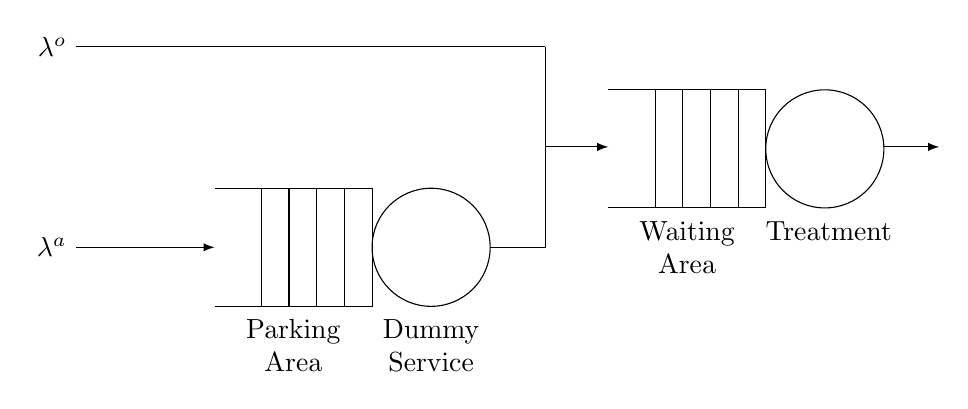
\begin{tikzpicture}[>=latex]
        % the rectangle with vertical rules (Queue 1)
        \draw (0,0) -- ++(2cm,0) -- ++(0,-1.5cm) -- ++(-2cm,0);
        \foreach \i in {1,...,4}
        \draw (2cm-\i*10pt,0) -- +(0,-1.5cm);
        
        % the circle (Queue 1)
        \draw (2.75,-0.75cm) circle [radius=0.75cm];

        % the rectangle with vertical rules (Queue 2)
        \draw (5,1.25) -- ++(2cm,0) -- ++(0,-1.5cm) -- ++(-2cm,0);
        \foreach \i in {1,...,4}
        \draw (7cm-\i*10pt,1.25) -- +(0,-1.5cm);

        % the circle (Queue 2)
        \draw (7.75,0.5) circle [radius=0.75cm];

        % the arrows and labels (Queue 1+2)
        \draw[-] (3.5,-0.75) -- +(20pt,0);
        \draw[<-] (0,-0.75) -- +(-50pt,0) node[left] {$\lambda^a$};
        \draw[->] (8.5,0.525) -- +(20pt,0);
        \node[align=center] at (1cm,-2cm) {Parking \\ Area};
        \node[align=center] at (2.75cm,-2cm) {Dummy \\ Service};
        \node[align=center] at (6cm,-0.75cm) {Waiting \\ Area};
        \node[align=center] at (7.8cm,-0.75cm) {Treatment \\ };
        
        \draw (4.2, 1.8) -- +(-169.5pt,0) node[left] {$\lambda^o$};
        \draw (4.2, 1.8) -- (4.2, -0.75);
        \draw[->] (4.2, 0.525) -- (5, 0.525);

    \end{tikzpicture}

\end{figure}

\begin{figure}[h]
    \centering
    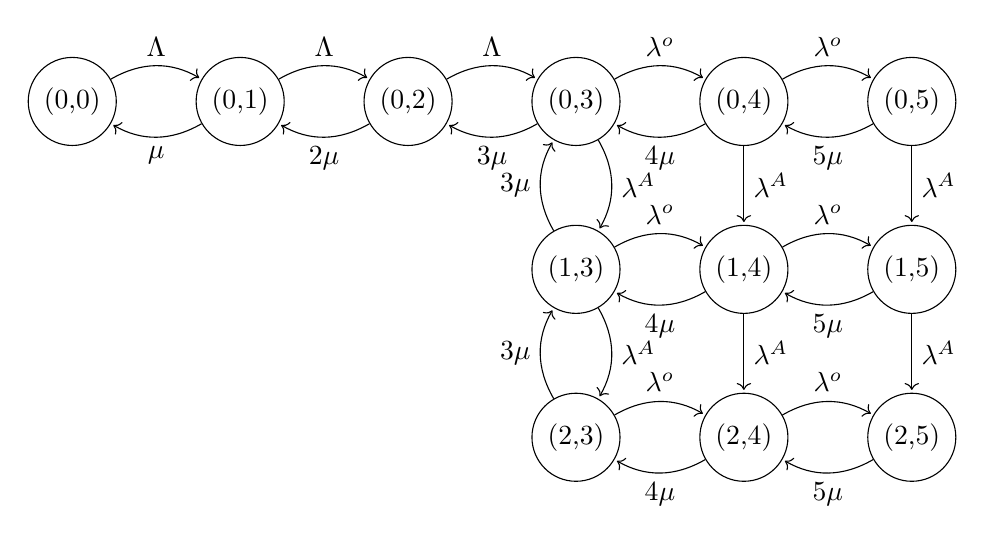
\begin{tikzpicture}[-, node distance = 1cm, auto]
        \node[state] (empty) {(0,0)};
        \node[state, right=of empty] (one) {(0,1)};
        \node[state, right=of one] (two) {(0,2)};
        \node[state, right=of two] (three) {(0,3)};
        \node[state, right=of three] (four) {(0,4)};
        \node[state, right=of four] (five) {(0,5)};

        \node[state, below=of three] (three_one) {(1,3)};
        \node[state, below=of three_one] (three_two) {(2,3)};
        \node[state, below=of four] (four_one) {(1,4)};
        \node[state, below=of four_one] (four_two) {(2,4)};
        \node[state, below=of five] (five_one) {(1,5)};
        \node[state, below=of five_one] (five_two) {(2,5)};



        \draw[every loop]
            (empty) edge[bend left] node {$\Lambda$} (one)
            (one) edge[bend left] node {$\mu$} (empty)
            (one) edge[bend left] node {$\Lambda$} (two)
            (two) edge[bend left] node {$2 \mu$} (one)
            (two) edge[bend left] node {$\Lambda$} (three)
            (three) edge[bend left] node {$3 \mu$} (two)
            (three) edge[bend left] node {$\lambda^o$} (four)
            (four) edge[bend left] node {$4 \mu$} (three)
            (four) edge[bend left] node {$\lambda^o$} (five)
            (five) edge[bend left] node {$5 \mu$} (four)
            (three) edge[bend left] node {$\lambda^A$} (three_one)
            (three_one) edge[bend left] node {$3 \mu$} (three)
            (three_one) edge[bend left] node {$\lambda^o$} (four_one)
            (four_one) edge[bend left] node {$4 \mu$} (three_one)
            (four_one) edge[bend left] node {$\lambda^o$} (five_one)
            (five_one) edge[bend left] node {$5 \mu$} (four_one)
            (four) edge node {$\lambda^A$} (four_one)
            % (four_one) edge[bend left] node {$\mu$} (four)
            (five) edge node {$\lambda^A$} (five_one)
            % (five_one) edge[bend left] node {$\mu$} (five)
            (three_one) edge[bend left] node {$\lambda^A$} (three_two)
            (three_two) edge[bend left] node {$3 \mu$} (three_one)
            (four_one) edge node {$\lambda^A$} (four_two)
            % (four_two) edge[bend left] node {$\mu$} (four_one)
            (five_one) edge node {$\lambda^A$} (five_two)
            % (five_two) edge[bend left] node {$\mu$} (five_one)
            (three_two) edge[bend left] node {$\lambda^o$} (four_two)
            (four_two) edge[bend left] node {$4 \mu$} (three_two)
            (four_two) edge[bend left] node {$\lambda^o$} (five_two)
            (five_two) edge[bend left] node {$5 \mu$} (four_two)
            ;       


    \end{tikzpicture}
    \caption{Markov chains} 
    \label{Markov_mini}
\end{figure}





\newpage
\begin{figure}
    \centering
    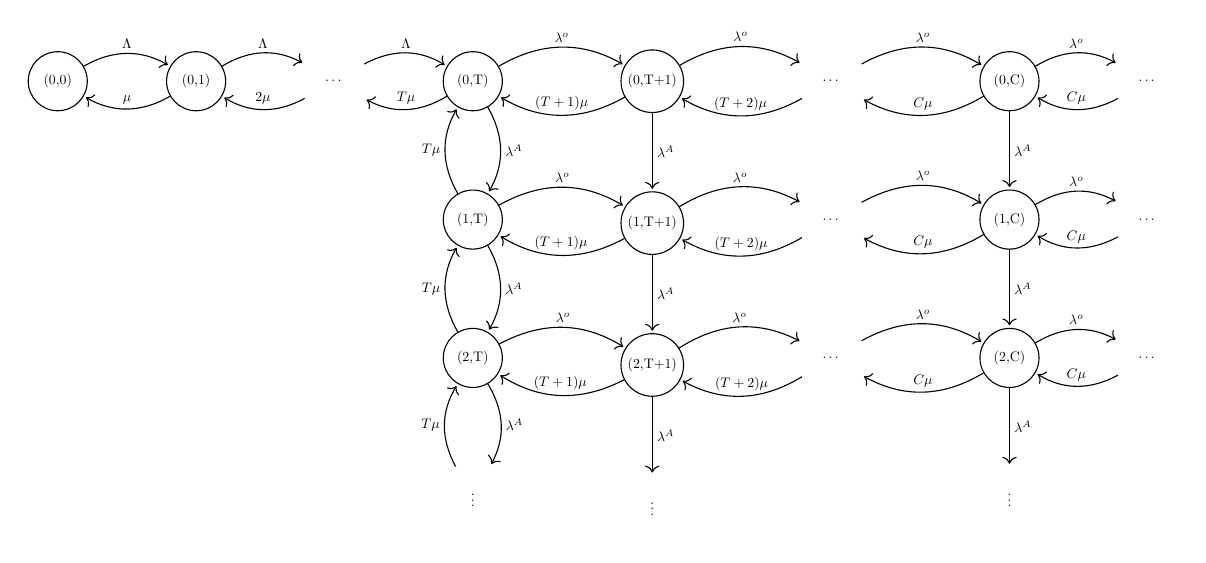
\begin{tikzpicture}[-, node distance = 1cm, auto, every node/.style={scale=0.5}]

        % Variables
        \tikzmath{
            let \altdist = 1.5cm;
            let \minsz = 1.5cm;
        }

        % First Line
        \node[state, minimum size=1.5cm] (zero) {(0,0)};
        \node[state, minimum size=1.5cm,  right=of zero] (one) {(0,1)};
        \node[draw=none, minimum size=1.5cm, right=of one] (two) {\dots};
        \node[state, minimum size=1.5cm, right=of two] (three) {(0,T)};
        \node[state, node distance = \altdist, minimum size=\minsz, right=of three] (four) {(0,T+1)};
        \node[draw=none, node distance = \altdist, minimum size=\minsz, right=of four] (five) {\dots};
        \node[state, node distance = \altdist, minimum size=\minsz, right=of five] (six) {(0,C)};
        \node[draw=none, minimum size=\minsz, right=of six] (seven) {\dots};

        % Second Line
        \node[state, minimum size=\minsz, below=of three] (three_one) {(1,T)};
        \node[state, minimum size=\minsz, below=of four] (four_one) {(1,T+1)};
        \node[draw=none, minimum size=\minsz, below=of five] (five_one) {\dots};
        \node[state, node distance = \altdist, minimum size=\minsz, right=of five_one] (six_one) {(1,C)};
        \node[draw=none, minimum size=\minsz, right=of six_one] (seven_one) {\dots};

        % Third Line
        \node[state, minimum size=\minsz, below=of three_one] (three_two) {(2,T)};
        \node[state, minimum size=\minsz, below=of four_one] (four_two) {(2,T+1)};
        \node[draw=none, minimum size=\minsz, below=of five_one] (five_two) {\dots};
        \node[state, node distance = \altdist, minimum size=\minsz, right=of five_two] (six_two) {(2,C)};
        \node[draw=none, minimum size=\minsz, right=of six_two] (seven_two) {\dots};

        % Fourth line
        \node[draw=none, minimum size=\minsz, below=of three_two] (three_three) {\vdots};
        \node[draw=none, minimum size=\minsz, below=of four_two] (four_three) {\vdots};
        \node[draw=none, minimum size=\minsz, below=of five_two] (five_three) {};
        \node[draw=none, node distance = \altdist, minimum size=\minsz, right=of five_three] (six_three) {\vdots};

        \draw[every loop]
            % First Horizontal Edges
            (zero) edge[bend left] node {$\Lambda$} (one)
            (one) edge[bend left] node [above] {$\mu$} (zero)
            (one) edge[bend left] node {$\Lambda$} (two)
            (two) edge[bend left] node [above] {$2 \mu$} (one)
            (two) edge[bend left] node {$\Lambda$} (three)
            (three) edge[bend left] node [above] {$T \mu$} (two)
            (three) edge[bend left] node {$\lambda^o$} (four)
            (four) edge[bend left] node [above] {$(T+1) \mu$} (three)
            (four) edge[bend left] node {$\lambda^o$} (five)
            (five) edge[bend left] node [above] {$(T+2) \mu$} (four)
            (five) edge[bend left] node {$\lambda^o$} (six)
            (six) edge[bend left] node [above] {$C\mu$} (five)
            (six) edge[bend left] node {$\lambda^o$} (seven)
            (seven) edge[bend left] node [above] {$C\mu$} (six)

            % Second Horizontal Edges
            (three_one) edge[bend left] node {$\lambda^o$} (four_one)
            (four_one) edge[bend left] node [above] {$(T+1) \mu$} (three_one)
            (four_one) edge[bend left] node {$\lambda^o$} (five_one)
            (five_one) edge[bend left] node [above] {$(T+2) \mu$} (four_one)
            (five_one) edge[bend left] node {$\lambda^o$} (six_one)
            (six_one) edge[bend left] node [above] {$C\mu$} (five_one)
            (six_one) edge[bend left] node {$\lambda^o$} (seven_one)
            (seven_one) edge[bend left] node [above] {$C\mu$} (six_one)

            % Third Horizontal Edges
            (three_two) edge[bend left] node {$\lambda^o$} (four_two)
            (four_two) edge[bend left] node [above] {$(T+1) \mu$} (three_two)
            (four_two) edge[bend left] node {$\lambda^o$} (five_two)
            (five_two) edge[bend left] node [above] {$(T+2) \mu$} (four_two)
            (five_two) edge[bend left] node {$\lambda^o$} (six_two)
            (six_two) edge[bend left] node [above] {$C\mu$} (five_two)
            (six_two) edge[bend left] node {$\lambda^o$} (seven_two)
            (seven_two) edge[bend left] node [above] {$C\mu$} (six_two)

            % First Vertical Edges
            (three) edge[bend left] node {$\lambda^A$} (three_one)
            (three_one) edge[bend left] node {$T \mu$} (three)
            (three_one) edge[bend left] node {$\lambda^A$} (three_two)
            (three_two) edge[bend left] node {$T\mu$} (three_one)
            (three_two) edge[bend left] node {$\lambda^A$} (three_three)
            (three_three) edge[bend left] node {$T\mu$} (three_two)

            % Second Vertical Edges
            (four) edge node {$\lambda^A$} (four_one)
            (four_one) edge node {$\lambda^A$} (four_two)
            (four_two) edge node {$\lambda^A$} (four_three)

            %Third Vertical Edges
            (six) edge node {$\lambda^A$} (six_one)
            (six_one) edge node {$\lambda^A$} (six_two)
            (six_two) edge node {$\lambda^A$} (six_three)
            ;       
    \end{tikzpicture}
    \caption{Markov chains} 
    \label{Markov_2}
\end{figure}

\begin{figure}
    \centering
    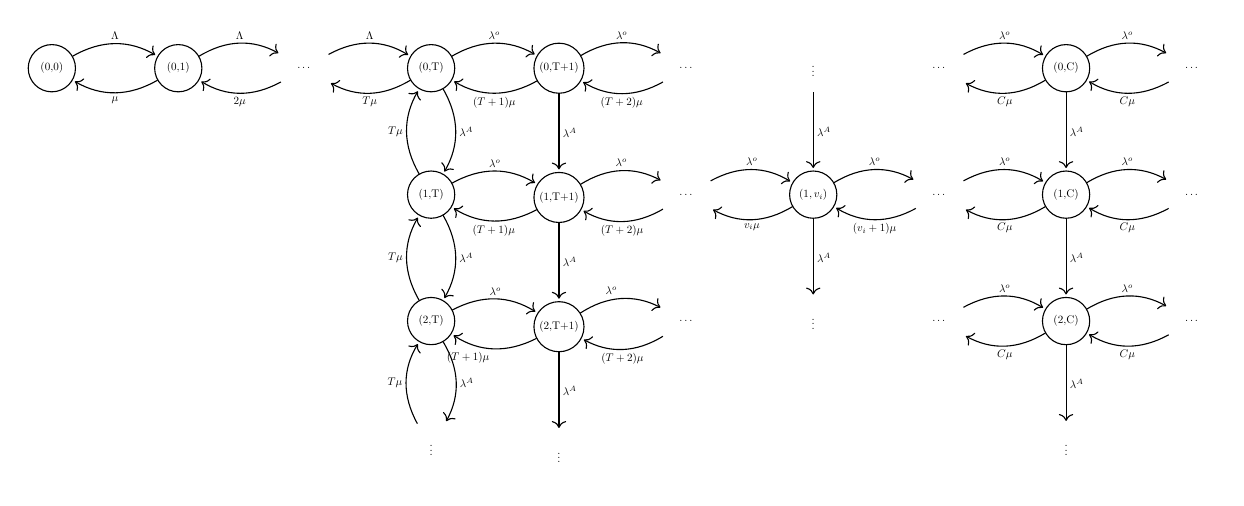
\begin{tikzpicture}[-, node distance = 1cm, auto, every node/.style={scale=0.4}]

        % Variables
        \tikzmath{
            let \altdist = 1cm;
            let \minsz = 1.5cm;
        }

        % First Line
        \node[state, minimum size=1.5cm] (zero) {(0,0)};
        \node[state, minimum size=1.5cm,  right=of zero] (one) {(0,1)};
        \node[draw=none, minimum size=1.5cm, right=of one] (two) {\dots};
        \node[state, minimum size=1.5cm, right=of two] (three) {(0,T)};
        \node[state, node distance = \altdist, minimum size=\minsz, right=of three] (four) {(0,T+1)};
        \node[draw=none, minimum size=\minsz, right=of four] (five) {\dots};
        \node[draw=none, minimum size=\minsz, right=of five] (six) {\vdots};
        \node[draw=none, minimum size=\minsz, right=of six] (seven) {\dots};
        \node[state, minimum size=\minsz, right=of seven] (eight) {(0,C)};
        \node[draw=none, minimum size=\minsz, right=of eight] (nine) {\dots};


        % Second Line
        \node[state, minimum size=\minsz, below=of three] (three_one) {(1,T)};
        \node[state, minimum size=\minsz, below=of four] (four_one) {(1,T+1)};
        \node[draw=none, minimum size=\minsz, below=of five] (five_one) {\dots};
        \node[state, node distance = \altdist, minimum size=\minsz, right=of five_one] (six_one) {$(1, v_i)$};
        \node[draw=none, minimum size=\minsz, right=of six_one] (seven_one) {\dots};
        \node[state, node distance = \altdist, minimum size=\minsz, right=of seven_one] (eight_one) {(1,C)};
        \node[draw=none, minimum size=\minsz, right=of eight_one] (nine_one) {\dots};
        

        % Third Line
        \node[state, minimum size=\minsz, below=of three_one] (three_two) {(2,T)};
        \node[state, minimum size=\minsz, below=of four_one] (four_two) {(2,T+1)};
        \node[draw=none, minimum size=\minsz, below=of five_one] (five_two) {\dots};
        \node[draw=none, node distance = \altdist, minimum size=\minsz, right=of five_two] (six_two) {\vdots};
        \node[draw=none, minimum size=\minsz, right=of six_two] (seven_two) {\dots};
        \node[state, node distance = \altdist, minimum size=\minsz, right=of seven_two] (eight_two) {(2,C)};
        \node[draw=none, minimum size=\minsz, right=of eight_two] (nine_two) {\dots};

        % Fourth line
        \node[draw=none, minimum size=\minsz, below=of three_two] (three_three) {\vdots};
        \node[draw=none, minimum size=\minsz, below=of four_two] (four_three) {\vdots};
        \node[draw=none, minimum size=\minsz, below=of five_two] (five_three) {};
        \node[draw=none, node distance = \altdist, minimum size=\minsz, right=of five_three] (six_three) {};
        \node[draw=none, node distance = \altdist, minimum size=\minsz, below=of eight_two] (eight_three) {\vdots};


        \draw[every loop]
            % First Horizontal Edges
            (zero) edge[bend left] node {$\Lambda$} (one)
            (one) edge[bend left] node {$\mu$} (zero)
            (one) edge[bend left] node {$\Lambda$} (two)
            (two) edge[bend left] node {$2 \mu$} (one)
            (two) edge[bend left] node {$\Lambda$} (three)
            (three) edge[bend left] node {$T \mu$} (two)
            (three) edge[bend left] node {$\lambda^o$} (four)
            (four) edge[bend left] node {$(T+1) \mu$} (three)
            (four) edge[bend left] node {$\lambda^o$} (five)
            (five) edge[bend left] node {$(T+2) \mu$} (four)
            % (five) edge[bend left] node {$\lambda^o$} (six)
            % (six) edge[bend left] node [above] {$C\mu$} (five)
            % (six) edge[bend left] node {$\lambda^o$} (seven)
            % (seven) edge[bend left] node [above] {$C\mu$} (six)
            (seven) edge[bend left] node {$\lambda^o$} (eight)
            (eight) edge[bend left] node {$C\mu$} (seven)
            (eight) edge[bend left] node {$\lambda^o$} (nine)
            (nine) edge[bend left] node {$C\mu$} (eight)

            % Second Horizontal Edges
            (three_one) edge[bend left] node {$\lambda^o$} (four_one)
            (four_one) edge[bend left] node {$(T+1) \mu$} (three_one)
            (four_one) edge[bend left] node {$\lambda^o$} (five_one)
            (five_one) edge[bend left] node {$(T+2) \mu$} (four_one)
            (five_one) edge[bend left] node {$\lambda^o$} (six_one)
            (six_one) edge[bend left] node {$v_i\mu$} (five_one)
            (six_one) edge[bend left] node {$\lambda^o$} (seven_one)
            (seven_one) edge[bend left] node {$(v_i+1)\mu$} (six_one)
            (seven_one) edge[bend left] node {$\lambda^o$} (eight_one)
            (eight_one) edge[bend left] node {$C\mu$} (seven_one)
            (eight_one) edge[bend left] node {$\lambda^o$} (nine_one)
            (nine_one) edge[bend left] node {$C\mu$} (eight_one)

            % Third Horizontal Edges
            (three_two) edge[bend left] node {$\lambda^o$} (four_two)
            (four_two) edge[bend left] node {$(T+1) \mu$} (three_two)
            (four_two) edge[bend left] node {$\lambda^o$} (five_two)
            (five_two) edge[bend left] node {$(T+2) \mu$} (four_two)
            % (five_two) edge[bend left] node {$\lambda^o$} (six_two)
            % (six_two) edge[bend left] node [above] {$C\mu$} (five_two)
            % (six_two) edge[bend left] node {$\lambda^o$} (seven_two)
            % (seven_two) edge[bend left] node [above] {$C\mu$} (six_two)
            (seven_two) edge[bend left] node {$\lambda^o$} (eight_two)
            (eight_two) edge[bend left] node {$C\mu$} (seven_two)
            (eight_two) edge[bend left] node {$\lambda^o$} (nine_two)
            (nine_two) edge[bend left] node {$C\mu$} (eight_two)

            % First Vertical Edges
            (three) edge[bend left] node {$\lambda^A$} (three_one)
            (three_one) edge[bend left] node {$T \mu$} (three)
            (three_one) edge[bend left] node {$\lambda^A$} (three_two)
            (three_two) edge[bend left] node {$T\mu$} (three_one)
            (three_two) edge[bend left] node {$\lambda^A$} (three_three)
            (three_three) edge[bend left] node {$T\mu$} (three_two)

            % Second Vertical Edges
            (four) edge node {$\lambda^A$} (four_one)
            (four_one) edge node {$\lambda^A$} (four_two)
            (four_two) edge node {$\lambda^A$} (four_three)

            % Third Vertical Edges
            (six) edge node {$\lambda^A$} (six_one)
            (six_one) edge node {$\lambda^A$} (six_two)
            % (six_two) edge node {$\lambda^A$} (six_three)

            % Fourth Vertical Edges
            (eight) edge node {$\lambda^A$} (eight_one)
            (eight_one) edge node {$\lambda^A$} (eight_two)
            (eight_two) edge node {$\lambda^A$} (eight_three)
            ;       
    \end{tikzpicture}
    \caption{Markov chains} 
    \label{Markov_3}
\end{figure}


\begin{figure}
    \centering
    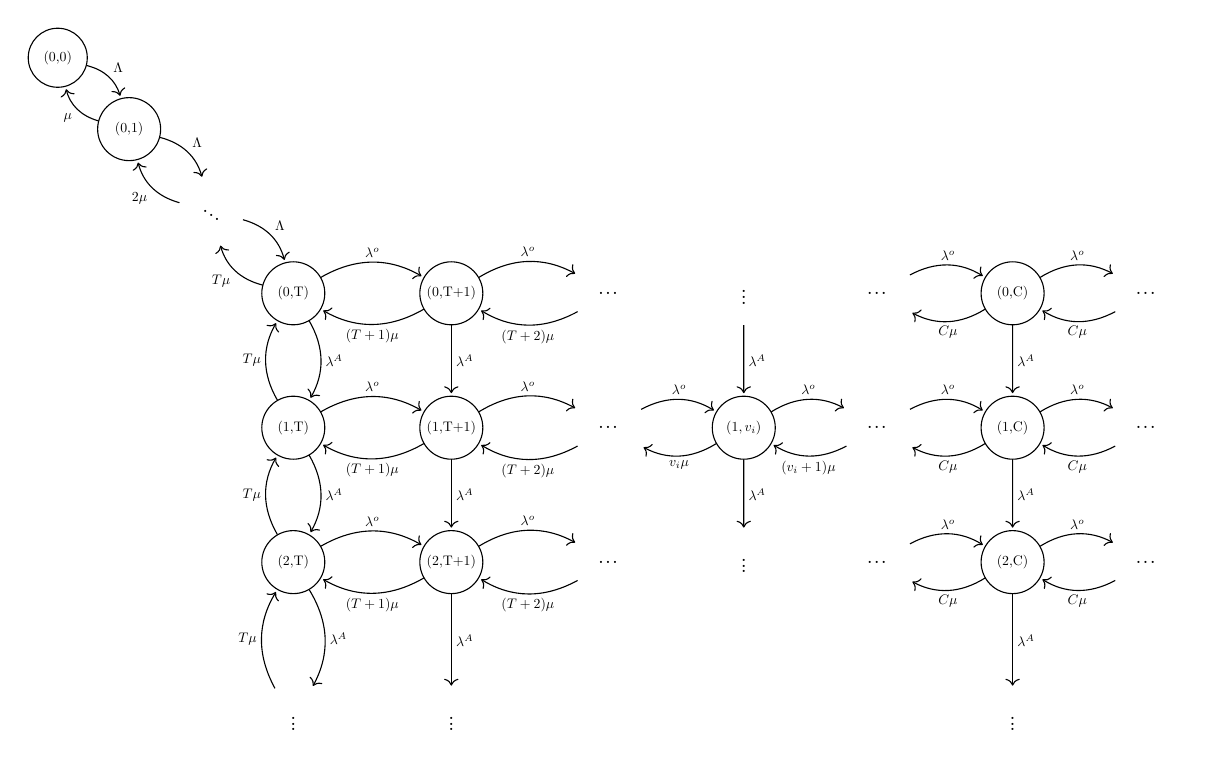
\begin{tikzpicture}[-, node distance = 0.9cm, auto, every node/.style={scale=0.5}]

        % Variables
        \tikzmath{
            let \initdist = 0.5cm;
            let \altdist = 1.2cm;
            let \minsz = 1.6cm;
            let \leftOne = -0.8;
            let \rightOne = 2.2;
            let \upOne = 0.8;
            let \downOne = -2.2;
            let \leftTwo = 2.25;
            let \rightTwo = 14.2;
            let \upTwo = -2.35;
            let \downTwo = -8.8;
        }

        % % Rectangle for S1
        % \draw[ultra thin, dashed] (\leftOne, \downOne) -- (\leftOne, \upOne);
        % \draw[ultra thin, dashed] (\leftOne, \upOne) -- (\rightOne, \upOne);
        % \draw[ultra thin, dashed] (\rightOne, \upOne) -- node {\Huge{$\quad S_1$}}(\rightOne, \downOne);
        % \draw[ultra thin, dashed] (\rightOne, \downOne) -- (\leftOne, \downOne);

        % % Rectangle for S2
        % \draw[ultra thin, dashed] (\leftTwo, \downTwo) -- node {\Huge{$S_2 \quad$}}(\leftTwo, \upTwo);
        % \draw[ultra thin, dashed] (\leftTwo, \upTwo) -- (\rightTwo, \upTwo);
        % \draw[ultra thin, dashed] (\rightTwo, \upTwo) -- (\rightTwo, \downTwo);
        % \draw[ultra thin, dashed] (\rightTwo, \downTwo) -- (\leftTwo, \downTwo);

        % First Line
        \node[state, minimum size=1.5cm] (zero) {(0,0)};
        \node[state, node distance = \initdist, minimum size=\minsz, below right=of zero] (one) {(0,1)};
        \node[draw=none, node distance = \initdist, minimum size=\minsz, below right=of one] (two) {\textbf{$\ddots$}};
        \node[state, node distance = \initdist, minimum size=\minsz, below right=of two] (three) {(0,T)};
        \node[state, node distance = \altdist, minimum size=\minsz, right=of three] (four) {(0,T+1)};
        \node[draw=none, node distance = \altdist, minimum size=\minsz, right=of four] (five) {\textbf{\dots}};
        \node[draw=none, minimum size=\minsz, right=of five] (six) {\textbf{\vdots}};
        \node[draw=none, minimum size=\minsz, right=of six] (seven) {\textbf{\dots}};
        \node[state, minimum size=\minsz, right=of seven] (eight) {(0,C)};
        \node[draw=none, minimum size=\minsz, right=of eight] (nine) {\textbf{\dots}};


        % Second Line
        \node[state, minimum size=\minsz, below=of three] (three_one) {(1,T)};
        \node[state, minimum size=\minsz, below=of four] (four_one) {(1,T+1)};
        \node[draw=none, minimum size=\minsz, below=of five] (five_one) {\textbf{\dots}};
        \node[state, minimum size=\minsz, right=of five_one] (six_one) {$(1, v_i)$};
        \node[draw=none, minimum size=\minsz, right=of six_one] (seven_one) {\textbf{\dots}};
        \node[state, minimum size=\minsz, right=of seven_one] (eight_one) {(1,C)};
        \node[draw=none, minimum size=\minsz, right=of eight_one] (nine_one) {\textbf{\dots}};
        

        % Third Line
        \node[state, minimum size=\minsz, below=of three_one] (three_two) {(2,T)};
        \node[state, minimum size=\minsz, below=of four_one] (four_two) {(2,T+1)};
        \node[draw=none, minimum size=\minsz, below=of five_one] (five_two) {\textbf{\dots}};
        \node[draw=none, minimum size=\minsz, right=of five_two] (six_two) {\textbf{\vdots}};
        \node[draw=none, minimum size=\minsz, right=of six_two] (seven_two) {\textbf{\dots}};
        \node[state, minimum size=\minsz, right=of seven_two] (eight_two) {(2,C)};
        \node[draw=none, minimum size=\minsz, right=of eight_two] (nine_two) {\textbf{\dots}};

        % Fourth line
        \node[draw=none, node distance = \altdist, minimum size=\minsz, below=of three_two] (three_three) {\textbf{\vdots}};
        \node[draw=none, node distance = \altdist, minimum size=\minsz, below=of four_two] (four_three) {\textbf{\vdots}};
        \node[draw=none, node distance = \altdist, minimum size=\minsz, below=of five_two] (five_three) {};
        \node[draw=none, node distance = \altdist, minimum size=\minsz, below=of six_two] (six_three) {};
        \node[draw=none, node distance = \altdist, minimum size=\minsz, below=of eight_two] (eight_three) {\textbf{\vdots}};


        \draw[every loop]
            % First Horizontal Edges
            (zero) edge[bend left] node {$\Lambda$} (one)
            (one) edge[bend left] node {$\mu$} (zero)
            (one) edge[bend left] node {$\Lambda$} (two)
            (two) edge[bend left] node {$2 \mu$} (one)
            (two) edge[bend left] node {$\Lambda$} (three)
            (three) edge[bend left] node {$T \mu$} (two)
            (three) edge[bend left] node {$\lambda^o$} (four)
            (four) edge[bend left] node {$(T+1) \mu$} (three)
            (four) edge[bend left] node {$\lambda^o$} (five)
            (five) edge[bend left] node {$(T+2) \mu$} (four)
            % (five) edge[bend left] node {$\lambda^o$} (six)
            % (six) edge[bend left] node [above] {$C\mu$} (five)
            % (six) edge[bend left] node {$\lambda^o$} (seven)
            % (seven) edge[bend left] node [above] {$C\mu$} (six)
            (seven) edge[bend left] node {$\lambda^o$} (eight)
            (eight) edge[bend left] node {$C\mu$} (seven)
            (eight) edge[bend left] node {$\lambda^o$} (nine)
            (nine) edge[bend left] node {$C\mu$} (eight)

            % Second Horizontal Edges
            (three_one) edge[bend left] node {$\lambda^o$} (four_one)
            (four_one) edge[bend left] node {$(T+1) \mu$} (three_one)
            (four_one) edge[bend left] node {$\lambda^o$} (five_one)
            (five_one) edge[bend left] node {$(T+2) \mu$} (four_one)
            (five_one) edge[bend left] node {$\lambda^o$} (six_one)
            (six_one) edge[bend left] node {$v_i\mu$} (five_one)
            (six_one) edge[bend left] node {$\lambda^o$} (seven_one)
            (seven_one) edge[bend left] node {$(v_i+1)\mu$} (six_one)
            (seven_one) edge[bend left] node {$\lambda^o$} (eight_one)
            (eight_one) edge[bend left] node {$C\mu$} (seven_one)
            (eight_one) edge[bend left] node {$\lambda^o$} (nine_one)
            (nine_one) edge[bend left] node {$C\mu$} (eight_one)

            % Third Horizontal Edges
            (three_two) edge[bend left] node {$\lambda^o$} (four_two)
            (four_two) edge[bend left] node [below] {$(T+1) \mu$} (three_two)
            (four_two) edge[bend left] node {$\lambda^o$} (five_two)
            (five_two) edge[bend left] node {$(T+2) \mu$} (four_two)
            % (five_two) edge[bend left] node {$\lambda^o$} (six_two)
            % (six_two) edge[bend left] node [above] {$C\mu$} (five_two)
            % (six_two) edge[bend left] node {$\lambda^o$} (seven_two)
            % (seven_two) edge[bend left] node [above] {$C\mu$} (six_two)
            (seven_two) edge[bend left] node {$\lambda^o$} (eight_two)
            (eight_two) edge[bend left] node {$C\mu$} (seven_two)
            (eight_two) edge[bend left] node {$\lambda^o$} (nine_two)
            (nine_two) edge[bend left] node {$C\mu$} (eight_two)

            % First Vertical Edges
            (three) edge[bend left] node {$\lambda^A$} (three_one)
            (three_one) edge[bend left] node {$T \mu$} (three)
            (three_one) edge[bend left] node {$\lambda^A$} (three_two)
            (three_two) edge[bend left] node {$T\mu$} (three_one)
            (three_two) edge[bend left] node {$\lambda^A$} (three_three)
            (three_three) edge[bend left] node {$T\mu$} (three_two)

            % Second Vertical Edges
            (four) edge node {$\lambda^A$} (four_one)
            (four_one) edge node {$\lambda^A$} (four_two)
            (four_two) edge node {$\lambda^A$} (four_three)

            % Third Vertical Edges
            (six) edge node {$\lambda^A$} (six_one)
            (six_one) edge node {$\lambda^A$} (six_two)
            % (six_two) edge node {$\lambda^A$} (six_three)

            % Fourth Vertical Edges
            (eight) edge node {$\lambda^A$} (eight_one)
            (eight_one) edge node {$\lambda^A$} (eight_two)
            (eight_two) edge node {$\lambda^A$} (eight_three)
            ;       
    \end{tikzpicture}
    \caption{Markov chains} 
    \label{Markov_4}
\end{figure}

\end{document}
